\documentclass[]{article}
\usepackage{lmodern}
\usepackage{amssymb,amsmath}
\usepackage{ifxetex,ifluatex}
\usepackage{fixltx2e} % provides \textsubscript
\ifnum 0\ifxetex 1\fi\ifluatex 1\fi=0 % if pdftex
  \usepackage[T1]{fontenc}
  \usepackage[utf8]{inputenc}
\else % if luatex or xelatex
  \ifxetex
    \usepackage{mathspec}
  \else
    \usepackage{fontspec}
  \fi
  \defaultfontfeatures{Ligatures=TeX,Scale=MatchLowercase}
\fi
% use upquote if available, for straight quotes in verbatim environments
\IfFileExists{upquote.sty}{\usepackage{upquote}}{}
% use microtype if available
\IfFileExists{microtype.sty}{%
\usepackage{microtype}
\UseMicrotypeSet[protrusion]{basicmath} % disable protrusion for tt fonts
}{}
\usepackage[margin=1in]{geometry}
\usepackage{hyperref}
\hypersetup{unicode=true,
            pdftitle={Tissue Weights for Muscle Tsc1 Knockout Mice},
            pdfauthor={Dave Bridges and Erin Stephenson},
            pdfborder={0 0 0},
            breaklinks=true}
\urlstyle{same}  % don't use monospace font for urls
\usepackage{color}
\usepackage{fancyvrb}
\newcommand{\VerbBar}{|}
\newcommand{\VERB}{\Verb[commandchars=\\\{\}]}
\DefineVerbatimEnvironment{Highlighting}{Verbatim}{commandchars=\\\{\}}
% Add ',fontsize=\small' for more characters per line
\usepackage{framed}
\definecolor{shadecolor}{RGB}{248,248,248}
\newenvironment{Shaded}{\begin{snugshade}}{\end{snugshade}}
\newcommand{\KeywordTok}[1]{\textcolor[rgb]{0.13,0.29,0.53}{\textbf{#1}}}
\newcommand{\DataTypeTok}[1]{\textcolor[rgb]{0.13,0.29,0.53}{#1}}
\newcommand{\DecValTok}[1]{\textcolor[rgb]{0.00,0.00,0.81}{#1}}
\newcommand{\BaseNTok}[1]{\textcolor[rgb]{0.00,0.00,0.81}{#1}}
\newcommand{\FloatTok}[1]{\textcolor[rgb]{0.00,0.00,0.81}{#1}}
\newcommand{\ConstantTok}[1]{\textcolor[rgb]{0.00,0.00,0.00}{#1}}
\newcommand{\CharTok}[1]{\textcolor[rgb]{0.31,0.60,0.02}{#1}}
\newcommand{\SpecialCharTok}[1]{\textcolor[rgb]{0.00,0.00,0.00}{#1}}
\newcommand{\StringTok}[1]{\textcolor[rgb]{0.31,0.60,0.02}{#1}}
\newcommand{\VerbatimStringTok}[1]{\textcolor[rgb]{0.31,0.60,0.02}{#1}}
\newcommand{\SpecialStringTok}[1]{\textcolor[rgb]{0.31,0.60,0.02}{#1}}
\newcommand{\ImportTok}[1]{#1}
\newcommand{\CommentTok}[1]{\textcolor[rgb]{0.56,0.35,0.01}{\textit{#1}}}
\newcommand{\DocumentationTok}[1]{\textcolor[rgb]{0.56,0.35,0.01}{\textbf{\textit{#1}}}}
\newcommand{\AnnotationTok}[1]{\textcolor[rgb]{0.56,0.35,0.01}{\textbf{\textit{#1}}}}
\newcommand{\CommentVarTok}[1]{\textcolor[rgb]{0.56,0.35,0.01}{\textbf{\textit{#1}}}}
\newcommand{\OtherTok}[1]{\textcolor[rgb]{0.56,0.35,0.01}{#1}}
\newcommand{\FunctionTok}[1]{\textcolor[rgb]{0.00,0.00,0.00}{#1}}
\newcommand{\VariableTok}[1]{\textcolor[rgb]{0.00,0.00,0.00}{#1}}
\newcommand{\ControlFlowTok}[1]{\textcolor[rgb]{0.13,0.29,0.53}{\textbf{#1}}}
\newcommand{\OperatorTok}[1]{\textcolor[rgb]{0.81,0.36,0.00}{\textbf{#1}}}
\newcommand{\BuiltInTok}[1]{#1}
\newcommand{\ExtensionTok}[1]{#1}
\newcommand{\PreprocessorTok}[1]{\textcolor[rgb]{0.56,0.35,0.01}{\textit{#1}}}
\newcommand{\AttributeTok}[1]{\textcolor[rgb]{0.77,0.63,0.00}{#1}}
\newcommand{\RegionMarkerTok}[1]{#1}
\newcommand{\InformationTok}[1]{\textcolor[rgb]{0.56,0.35,0.01}{\textbf{\textit{#1}}}}
\newcommand{\WarningTok}[1]{\textcolor[rgb]{0.56,0.35,0.01}{\textbf{\textit{#1}}}}
\newcommand{\AlertTok}[1]{\textcolor[rgb]{0.94,0.16,0.16}{#1}}
\newcommand{\ErrorTok}[1]{\textcolor[rgb]{0.64,0.00,0.00}{\textbf{#1}}}
\newcommand{\NormalTok}[1]{#1}
\usepackage{longtable,booktabs}
\usepackage{graphicx,grffile}
\makeatletter
\def\maxwidth{\ifdim\Gin@nat@width>\linewidth\linewidth\else\Gin@nat@width\fi}
\def\maxheight{\ifdim\Gin@nat@height>\textheight\textheight\else\Gin@nat@height\fi}
\makeatother
% Scale images if necessary, so that they will not overflow the page
% margins by default, and it is still possible to overwrite the defaults
% using explicit options in \includegraphics[width, height, ...]{}
\setkeys{Gin}{width=\maxwidth,height=\maxheight,keepaspectratio}
\IfFileExists{parskip.sty}{%
\usepackage{parskip}
}{% else
\setlength{\parindent}{0pt}
\setlength{\parskip}{6pt plus 2pt minus 1pt}
}
\setlength{\emergencystretch}{3em}  % prevent overfull lines
\providecommand{\tightlist}{%
  \setlength{\itemsep}{0pt}\setlength{\parskip}{0pt}}
\setcounter{secnumdepth}{5}
% Redefines (sub)paragraphs to behave more like sections
\ifx\paragraph\undefined\else
\let\oldparagraph\paragraph
\renewcommand{\paragraph}[1]{\oldparagraph{#1}\mbox{}}
\fi
\ifx\subparagraph\undefined\else
\let\oldsubparagraph\subparagraph
\renewcommand{\subparagraph}[1]{\oldsubparagraph{#1}\mbox{}}
\fi

%%% Use protect on footnotes to avoid problems with footnotes in titles
\let\rmarkdownfootnote\footnote%
\def\footnote{\protect\rmarkdownfootnote}

%%% Change title format to be more compact
\usepackage{titling}

% Create subtitle command for use in maketitle
\newcommand{\subtitle}[1]{
  \posttitle{
    \begin{center}\large#1\end{center}
    }
}

\setlength{\droptitle}{-2em}

  \title{Tissue Weights for Muscle Tsc1 Knockout Mice}
    \pretitle{\vspace{\droptitle}\centering\huge}
  \posttitle{\par}
    \author{Dave Bridges and Erin Stephenson}
    \preauthor{\centering\large\emph}
  \postauthor{\par}
      \predate{\centering\large\emph}
  \postdate{\par}
    \date{2019-02-08}


\begin{document}
\maketitle

{
\setcounter{tocdepth}{2}
\tableofcontents
}
\section{Purpose}\label{purpose}

To determine tissue weights at sacrifice for fat pads and muscle tissues

\section{Experimental Details}\label{experimental-details}

At sacrifice, after a 16h fast data were entered and collected in the
raw data sheet

These data can be found in
\textbf{/Users/davebrid/Documents/GitHub/TissueSpecificTscKnockouts/Mouse
Data/Muscle Tsc1 Knockout/NCD} in a file named \textbf{Sacrifice
Data.csv}. This script was most recently updated on \textbf{Thu Feb 28
13:58:44 2019}.

\section{Analysis}\label{analysis}

\begin{longtable}[]{@{}lrrrrr@{}}
\toprule
Sex & GonadalWAT\_mean.na & InguinalWAT\_mean.na & Quadriceps\_mean.na &
TricepsSurae\_mean.na & Heart\_mean.na\tabularnewline
\midrule
\endhead
Female & 0.492 & 0.316 & 0.166 & 0.132 & 0.107\tabularnewline
Female & 0.101 & 0.076 & 0.142 & 0.121 & 0.122\tabularnewline
Male & 0.792 & 0.574 & 0.224 & 0.172 & 0.144\tabularnewline
Male & 0.181 & 0.116 & 0.192 & 0.156 & 0.132\tabularnewline
\bottomrule
\end{longtable}

\begin{longtable}[]{@{}lrrrrr@{}}
\toprule
Sex & GonadalWAT\_length & InguinalWAT\_length & Quadriceps\_length &
TricepsSurae\_length & Heart\_length\tabularnewline
\midrule
\endhead
Female & 53 & 53 & 53 & 53 & 53\tabularnewline
Female & 8 & 8 & 8 & 8 & 8\tabularnewline
Male & 25 & 25 & 25 & 25 & 25\tabularnewline
Male & 7 & 7 & 7 & 7 & 7\tabularnewline
\bottomrule
\end{longtable}

\subsection{Fat Pad Weights}\label{fat-pad-weights}

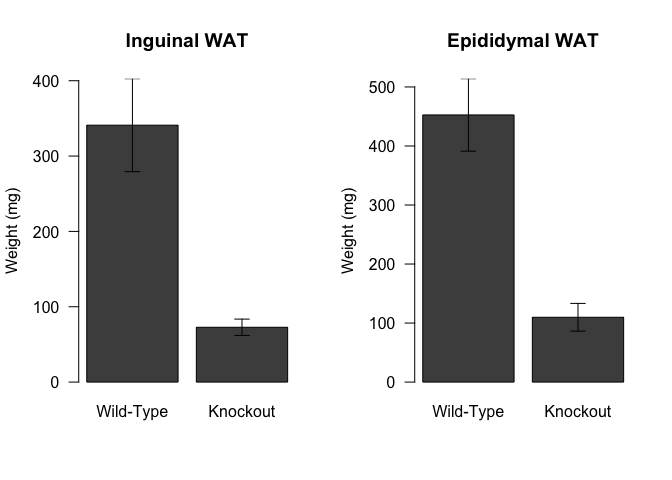
\includegraphics{figures/wat-weights-1.png}
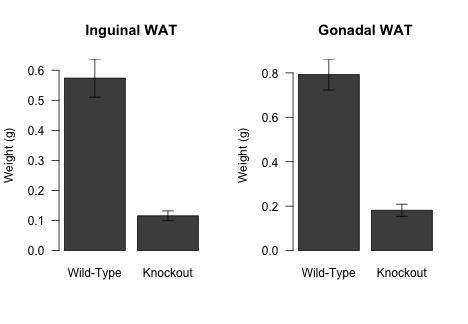
\includegraphics{figures/wat-weights-2.png}

For the male mice, the fat pads were reduced in weight:

\begin{longtable}[]{@{}lrrrr@{}}
\caption{Changes in Gonadal Fat Pad Weights}\tabularnewline
\toprule
Sex & Wild-Type & Knockout & Difference & Pct.Difference\tabularnewline
\midrule
\endfirsthead
\toprule
Sex & Wild-Type & Knockout & Difference & Pct.Difference\tabularnewline
\midrule
\endhead
Female & 0.492 & 0.101 & 0.391 & 79.5\tabularnewline
Male & 0.792 & 0.181 & 0.611 & 77.1\tabularnewline
\bottomrule
\end{longtable}

\begin{longtable}[]{@{}lrrrr@{}}
\caption{Changes in Inguinal Fat Pad Weights}\tabularnewline
\toprule
Sex & Wild-Type & Knockout & Difference & Pct.Difference\tabularnewline
\midrule
\endfirsthead
\toprule
Sex & Wild-Type & Knockout & Difference & Pct.Difference\tabularnewline
\midrule
\endhead
Female & 0.316 & 0.076 & 0.240 & 75.9\tabularnewline
Male & 0.574 & 0.116 & 0.458 & 79.8\tabularnewline
\bottomrule
\end{longtable}

\begin{longtable}[]{@{}llrr@{}}
\caption{Shapiro-Wilk Tests for each group}\tabularnewline
\toprule
Sex & Knockout & InguinalWAT\_shapiro.p &
GonadalWAT\_shapiro.p\tabularnewline
\midrule
\endfirsthead
\toprule
Sex & Knockout & InguinalWAT\_shapiro.p &
GonadalWAT\_shapiro.p\tabularnewline
\midrule
\endhead
Female & FALSE & 0.000 & 0.000\tabularnewline
Female & TRUE & 0.703 & 0.975\tabularnewline
Male & FALSE & 0.400 & 0.172\tabularnewline
Male & TRUE & 0.856 & 0.319\tabularnewline
\bottomrule
\end{longtable}

\begin{longtable}[]{@{}lrrrr@{}}
\caption{Pairwise tests for effects of knockout on Inguinal WAT
weights.}\tabularnewline
\toprule
Sex & Levene & Mann.Whitney & Welch & Student\tabularnewline
\midrule
\endfirsthead
\toprule
Sex & Levene & Mann.Whitney & Welch & Student\tabularnewline
\midrule
\endhead
Female & 0.018 & 0.001 & 0 & 0.007\tabularnewline
Male & 0.008 & 0.000 & 0 & 0.002\tabularnewline
\bottomrule
\end{longtable}

\begin{longtable}[]{@{}lrrrr@{}}
\caption{Pairwise tests for effects of knockout on Gonadal WAT
weights.}\tabularnewline
\toprule
Sex & Levene & Mann.Whitney & Welch & Student\tabularnewline
\midrule
\endfirsthead
\toprule
Sex & Levene & Mann.Whitney & Welch & Student\tabularnewline
\midrule
\endhead
Female & 0.016 & 0 & 0 & 0.007\tabularnewline
Male & 0.009 & 0 & 0 & 0.000\tabularnewline
\bottomrule
\end{longtable}

For the male mice, normality can be assumed, but not equal variance, so
a Welch's t-test is used, which had a p-value of 9.802×
10\textsuperscript{-7} for inguinal WAT and 4.917×
10\textsuperscript{-8} for gonadal WAT.

\subsection{Muscle Weights}\label{muscle-weights}

\begin{figure}
\centering
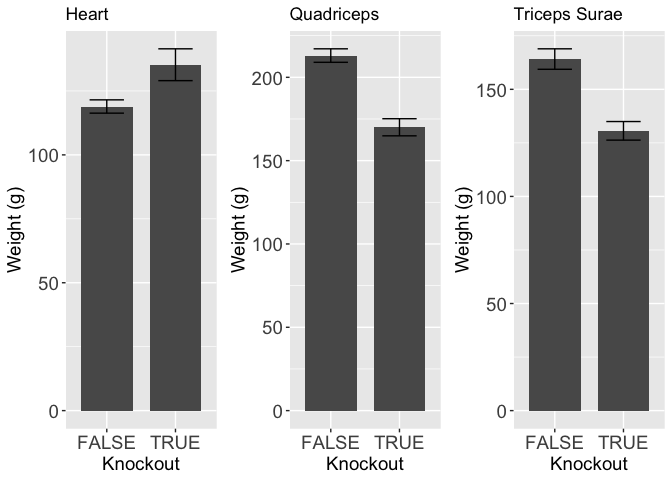
\includegraphics{figures/muscle-weights-1.png}
\caption{Weights of Muscle Depots at Sacrifice}
\end{figure}

\section{Session Information}\label{session-information}

\begin{Shaded}
\begin{Highlighting}[]
\KeywordTok{sessionInfo}\NormalTok{()}
\end{Highlighting}
\end{Shaded}

\begin{verbatim}
## R version 3.5.0 (2018-04-23)
## Platform: x86_64-apple-darwin15.6.0 (64-bit)
## Running under: macOS  10.14.2
## 
## Matrix products: default
## BLAS: /Library/Frameworks/R.framework/Versions/3.5/Resources/lib/libRblas.0.dylib
## LAPACK: /Library/Frameworks/R.framework/Versions/3.5/Resources/lib/libRlapack.dylib
## 
## locale:
## [1] en_US.UTF-8/en_US.UTF-8/en_US.UTF-8/C/en_US.UTF-8/en_US.UTF-8
## 
## attached base packages:
## [1] stats     graphics  grDevices utils     datasets  methods   base     
## 
## other attached packages:
##  [1] car_3.0-2          carData_3.0-2      forcats_0.3.0     
##  [4] gridExtra_2.3      ggplot2_3.1.0      RColorBrewer_1.1-2
##  [7] bindrcpp_0.2.2     readr_1.3.1        dplyr_0.7.8       
## [10] tidyr_0.8.2        knitr_1.21        
## 
## loaded via a namespace (and not attached):
##  [1] zip_1.0.0         Rcpp_1.0.0        cellranger_1.1.0 
##  [4] pillar_1.3.1      compiler_3.5.0    highr_0.7        
##  [7] plyr_1.8.4        bindr_0.1.1       tools_3.5.0      
## [10] digest_0.6.18     evaluate_0.12     tibble_2.0.0     
## [13] gtable_0.2.0      pkgconfig_2.0.2   rlang_0.3.1      
## [16] openxlsx_4.1.0    cli_1.0.1         curl_3.2         
## [19] yaml_2.2.0        haven_2.0.0       xfun_0.4         
## [22] rio_0.5.16        withr_2.1.2       stringr_1.3.1    
## [25] hms_0.4.2         grid_3.5.0        tidyselect_0.2.5 
## [28] data.table_1.11.8 glue_1.3.0        R6_2.3.0         
## [31] fansi_0.4.0       readxl_1.2.0      foreign_0.8-71   
## [34] rmarkdown_1.11    purrr_0.2.5       magrittr_1.5     
## [37] scales_1.0.0      htmltools_0.3.6   abind_1.4-5      
## [40] assertthat_0.2.0  colorspace_1.3-2  labeling_0.3     
## [43] utf8_1.1.4        stringi_1.2.4     lazyeval_0.2.1   
## [46] munsell_0.5.0     crayon_1.3.4
\end{verbatim}


\end{document}
